\documentclass{article}
\usepackage{graphicx} % Required for inserting images
\usepackage{natbib}
\usepackage{amsmath}
\usepackage{url} 
\usepackage[hidelinks]{hyperref}
\usepackage[T1]{fontenc}
\usepackage{mathpazo,euler}
\usepackage[scaled=0.9]{DejaVuSans}
\usepackage[utf8]{inputenc}
\usepackage{listings}
\usepackage{tabularx}
\usepackage{amsfonts}
\usepackage{booktabs}
\usepackage{siunitx}
\usepackage{geometry}

\geometry{margin=1.5in}
\lstset{basicstyle=\ttfamily}
%\documentclass[11pt]{article}
\setlength{\parskip}{1em} % 1em is an example value; adjust as needed
\bibliographystyle{abbrvnat}
\setcitestyle{authoryear,open={(},close={)}} % Citation-related commands

%\title{First Year Paper}
\title{First Year Paper} % Add your subtitle here

%\subtitle(Advisor: Moisés Expósito Alonso)
\author{Tatiana Bellagio \\ Advisor: Moisés Expósito Alonso}
\date{November 2023}
\begin{document}

\maketitle

\tableofcontents
\newpage % Starts a new page after the table of contents

\section{Introduction}
\subsection{Shift, Adapt or Perish}
When species face environmental changes that displace them from their ecological niche, there are only three possible outcomes: shift their geographical distribution to track suitable environments, adapt to the new imposed conditions, or face death or even extinction. Adaptation refers to the process by which a population becomes better suited to the new environment through changes in its genetic makeup. In the face of anthropogenic-generated climate and biodiversity crises environments are changing faster than ever (IPCC 2018; IPBES 2019) and adaptation through evolution must keep up to avoid extinction. In this context, understanding rapid eco-evolutionary dynamics has becomes more important than ever \citep{Waldvogel2020-dh, Palumbi2002-li, Stockwell2003-da}. 

\subsection{But what is rapid evolution?}
Evolution has been historically thought as a slow and gradual process occurring over extensive timescales, often spanning thousands to millions of years. However, genetically based rapid phenotypic changes have been shown to be pervasive in nature. The famous peppered moth \citep{Cook2013-bs}, insecticide resistance in Drosophila \citep{Daborn2002-is}, color of field mice \citep{Vignieri2010-if}, beak size in Darwin’s finches \citep{Grant2008-uc}, guppies in Trinidad \citep{Kemp2009-ji}, and Anolis lizards \citep{Losos2009-vq} and the evolved resistance to agricultural products in  200  plant species (Weedscience.org, 1993). 

Rapid evolution, can be defined by the number of generations in which a genetic change can be foreseen, but also as the convergence of ecological and evolutionary times \citep{Hairston2005-qo}. This highlights the importance of rapid evolution as one of the more applied domains within evolutionary biology. Coupled with advances in genome sequencing techonology that have led to an increase in the genomic data on non-model organisms, the understanding of eco-evolutionary dyamics have the potential to addres urgent ecological and conservation issues. Understanding and predicting the pace and direction of evolutionary changes can inform conservation strategies and management practices.  (Hoffmann  et al. 2015; Coulson et al. 2017; Bay et al. 2017a). 

As highlighted in \citep{Yamamichi2022-yj} short term eco-evolutionary dynamics, despite its inherent interdisciplinary nature, have been mostly studied solely from an ecological perspective and tended to focus on adaptation at the phenotypic level without considering the genetic part of the evolutionary process. More studies are needed in the evolutionary aspect of rapid adaptation to understand intertwined processes and to make more precise predictions.

\subsection{Trait architecture and adaptation}

Discussions concerning  how and where adaptive loci are distribute across the genome comes a long way. Since Darwin (Darwin 1859) and Huxley (Huxley 1860) there has been debates about whether the nature of adaptation is characterized by incremental, subtle variations in many loci or by abrupt changes on only a few of them. Even though, genetic architecture now spans a broader spectrum of concept ranging from pleiotropy to ploidy, these were the first debates surronding the quesiton  of what is the genetic architectures underlying adaptive processes. Compelling evidence shows that both cases can be true, and that there is considerable heterogeneity in architectures among adaptive traits \citep{Orr1992-xj, Orr1998-pr}. 

The implications of genetic architecture in the populations' evolutionary dyanmics have been widely documented. One example would be genetic architecture working as a buffer for adaptive alleles through dominance \citep{Yamamichi2017-uj}, or how the number of loci affecting reproductive incompatibility determines the outcome of the speciation processes \citep{Orr1996-eq}, and many more listed in \citep{Bertram2019-sg}. But, focusing on one key genetic architecture parameter in the adapation processes, two qualitative and timely diferent waves of research can be described. The first one, rooted on traditional population genetics focused on selective sweeps wherein adaptation depdnedn on only one or a few adaptive loci. The second wave, came with the advent of newer sequencing technologies and statistical methodologies showing that polygenic adaptation was pervasive. Since then, there has been major interest in the evolutionary dynamics of polygenic adaptation \citep{John2020-xc}  \citep{Jain2017-mb}, \citep{Barghi2020-aa} \citep{Hayward2021-ji, Stetter2018-st, Thornton2019-ww},  \citep{Hollinger2019-lb}. 

Nevertheless, all these works follow and old evolutionary view, spanning long time periods and extending over hundreds or thousands of generations and relying on a tremendous amount of de-novo mutation. As shown by \citep{Orr2008-jl}, adaptation to big environmental challenges over short periods can be difficult when relying on new mutations and populations will often decline to extinction. Oppositely, short term evolutionary dynamics may be more constrained by the limited amount of standing genetic variation \citep{Barrett2008-tj}. The implication of different trait genetic architectures from standing genetic variation on the dynamics of rapid evolution has not been yet explored. 

\subsection{How can we study rapid evolutionary dynamics? }

\subsubsection{Experiments}
On one hand, Evolve and Resequence experiments (E\&R) \citep{Schlotterer2015-yz}, are a well establish methodology in evolutionary biology. They combine the principles of experimental evolution with sequencing techniques, and consist on applying selective pressures in controlled environments and then pool sequencing the evolving populations over time. Some succesful examples inlcude \citep{Bergland2014-ud, Kapun2021-cd, Rudman2022-uc}. E\&R are particularly well-suited to study rapid evolution because they allow to observe evolutionary changes over relatively short periods and then, genomic scans are ussully used to identify genomic regions responsible for populations adaptation. For example \citep{Bergland2014-ud} was able to identify adaptive allele shifting seasonally in Drosophila populations. 

On the other hand, one of the most widely used experimental designs to find signals of local adaptation are common garden. Common gardens consist of growing individuals from different populations in the same set of controlled environments. By controlling the environment, any differences observed among populations are likely due to genetic variation. Some succesful examples are \citep{Exposito-Alonso2019-hs, Lepais2014-za}. A combined approach of (E\&R) and common garden experiments could be unusually powerful to identify the genomic regions responsable for climatic adaptation and to better understand rapid evolutionary dynamics. With this in mind, a multi generation and globally distributed common garden experiments was conducted, where 34 founder \textit{Arabidopsis thaliana} populations where planted and resequence over 4 years (\url{http://grene-net.org/}). Grene-net is the first of its kind, and the potentiality os this approach to study rapid evolutionary dynamics and the genomic regions responsible for cliamte adaptation needs to be explored. 

\subsubsection{Simulations}
In nature, selection forces are pervasive, and populations are simultaneosuly imposed to selective pressure acting on multiple traits spanning a range of genetic architectures, making it difficult to disentangle particular relationships. In this sense,  a way of disecting the complexity imposed in the real world, is through simulations. Forward in time individual based genetic simulations represent a powerful tool that allow the manipulation of known relevant parameters to get a deep understanding of key factors influencing evolutionary dynamics and outcomes. Simulations can allow us to not only understand how key parameters can affect the evolutionary processes, but also replicate real experiments to build a null hypothesis and generate expected results about the real world.  Finally, simulation outputs also allow the exploration of different statistical approaches to analyse real experimental data and evaluate the detectability of the signals we are looking for, like causal loci related to the adaptation process. 

\subsection{Detecting adaptive loci after rapid evolution}
Experimental evolution can allow us to detect genomic regions responsible for adaption to the new imposed condition. This is of extreme values, since this can have direct application for genetically targeting natural populations at extintion risk. But detecting loci underlying an adaption process is not a trivial task and has been evolving over the years. 

\subsubsection{Genome scans}
The genomic footprints of an adaptive process can be one of three types: hard sweeps, soft sweeps, and polygenic signals. These patterns will depend on the genetic architecture of the original adaptive trait. Historically, most selection scans have focused on detecting hard sweep (cite) because they align with a classical population genetic view and due to their discernible genetic pattern, a diversity reduction at the selected region compare to rest of the genome. More than a decade ago, Pritchard and Di Rienzo already highlighted that the vision of adaptation that proceeds by selective sweeps at key loci is too limited, and a more polygenic view coming from the field of quantitative genetics should be incorporated \citep{Pritchard2010-bv}. After this, with the advent of genomic datasets that can identify many variants with small
effect sizes, more efforts have been focus on detecting polygenic signal of adaptation \citep{Berg2014-zl} Pritchard et al. (2010); Sella and Barton (2019); Barghi et al. (2020); Fagny and Austerlitz (2021) \citep{Stephan2016-tx}

\subsubsection{Incorporating traits to the equation} 
Other fields, different from evolutionary biology, have been hihgly invested on identifying genomic regions associated with traits of interest. Wide Association Studies (GWAS) comes from human genetics and have been traditionally used  to find associations between specific genetic variants and traits or deseases. For these models, the predictor varaible is the individual's genetics, and the dependent variable is the trait value, this set up highlights the vision of the trait as an outcome of the genetic variants each individual carries. As disseases can be considered traits, fitness can be considered the sum of many traits, and these approaches can be used in the realm of evolutionary biology to find the loci responsible for these complex trait, adaptability in a given environment. 

\subsubsection{Incorporating environmental forces to the equation}
Finally, if we think of the environment as the sum of selective forces modeling the genomes under its presence, we could then incorporate the environment to enhance the detection of adaptive loci. Here, we enter the field of the so called genome environmental association studies. These approaches make the assumption that the distribution of alleles across space is a function of adaptation to contemporary environments, so each population is adapted to local conditions. More concretely, ff we assume that certain loci are responsable for adaptation to certain environemntal variable, we would expect to find a linear relationship between an environmental gradient and the allele frequencies of populations situated across that gradient. This approach has been used to developed different software including LFMM \citep{Frichot2013-mg}, Bayenv \citep{Gunther2013-fw}, and an expanded implementation of bayenv core model in Baypass \citep{Gautier2015-lp}. For these models the predictor variable is the environment and the dependent variable are the diferent allele frequencies, which higlights a different view of populations genetics as outcome of the environmental forces they are exposes.

\subsection{What is new?}
Since the relationship between different genetic architectures and the dynamics of rapid evolution across an environemntal gradient has not been yet exhaustively explored, we decided to conduct a set of simulations to achieve this. Furthermore, inspired by the Grene-Net project we decided to tailor our simulations on this real experiment so that the outcomes could also be used as ground truth for benchmarking and setting realistic expectations regarding the detectability of adaptive loci across various genetic architectures in the real data. 

Hence, this project aims to answer two main questions: 
\begin{itemize}
    \item Are rapid evolutionary dynamic different when the adaptive trait has a range of different genetic architectures? 
    \item Can we then detect the loci encoding the adaptive traits after a rapid evolution process?
\end{itemize}

\section{Methods}
\subsection{Simulations}

Simulation software
We used SLiM \citep{Haller2019-oj} for running a total of 189000 independent forward in time genetic simulations based on all combination of parameters plus replicated.  Each simulation represents a single population monitored for 10 generations. SLiM uniquely allowed us to have flexibility to simulate all the parameters below indicated, model specifics to \textit{A. thaliana} biology and work with tree sequences structures to achieve our goals in a computational efficient fashon. 

\subsubsection{Genetic diversity}
Because standing genetic variation is the subtract of rapid evolutionary changes rather than de-novo introduced genetic diversity via mutations, and to make our simulations more realistic we decided to work with real standing genetic variation. Since we were also interested in using this set of simulations as ground truth for the Grene-Net project we decided to use the genetic information from its founder populations. The founder population for all simulations consisted of a pool of 2310 individuals representing 231 different ecotypes coming from divergent climates across the world (full table of ecotypes in suplementary information), making it a highly diverse pool of individuals. 

\subsubsection{Trait genetic architecture}
We decided to model only one trait in which selection would act. We defined the trait genetic architecture based on three key parameters: polygenictiy, initial allele frequency and effect size. Polygenicity is defined as the total number of loci contributing to the trait value, and we calculated traits with 7 different levels for it. \ref{simulation_parameters_table}). We also built traits which encoding loci had 6 different ranges of initial allele frequency (Table \ref{simulation_parameters_table}). Finally the the effect size of each contributing loci was drawn from \( \sim N(0, 2) \) for all simulations

\subsubsection{Genetic value, heritability, environmental variance, and phenotype}

We used the additive genetic model for calculating the genetic value of each individual, such that \\ $A_n=\sum a_i$, where $A_n$ is the genetic value of the individual $n$ and \( a_i \) represents the effect size of the \( i \)-th contributing locus. We simulated 5 different levels of heritability for the trait (Table \ref{simulation_parameters_table}). For each simulation, using the breeders equation, we calculated:
\[
VE = \frac{VA - h^2 \cdot VA}{h^2}
\]
where \( VE \) is the environmental variance, \( VA \) represents the genetic variance from the given population \( VA = \text{Var}\left(\sum A_n\right) \), and \( h^2 \) is the heritability value for the given simulation. Once we had the value of \( VE \) we drew random samples of environmental noise (\( en \)) for each individual \( en_n \sim N(0, VE) \)to then calculate the phenotypic trait value of each individual by \( y_n = A_n+ en_n \). For each simulation we obtain the standard deviation and mean of the initial population to then use those values to standarize the phenotypes each generation before the fitness calculation.


\subsubsection{Selection}
We simulated two types of selection forces, stabilizing selection and directional selection defined by new optimum in a gradient of distances from the initial population phenotype mean. This double selection regimens, allowed us to investigate the relevance of different genetic architectures in a multiplicity of selection regimens, and understand where each parameters would have particular importance. 
\subsubsubsection{Stabilizing Selection}
Each individual n was subjected to stabilizing selection based on their phenotypic value with the formula:
\[
\text{Fitness}_\text{n} = \exp\left(-0.5 \times \frac{(\text{Phenotype}_\text{n} - {\text{Optimum phenotype}_\text{k}})^2}{\text{V}_\text{s}}\right)
\]
Were $\text{Optimum phenotype}_\text{k}$ refers to the optimum phenotype at the k environment and $\text{V}_\text{s}$ represent the strength of stabilizing selection. We simulated 4 different levels of selection \ref{fig:parameters}. Finally,  $\text{Fitness}_\text{n}$ would serve as a probability of survival of the individual n to the next generation.

\subsubsubsection{Environmental gradient - Directional Selection}
We simulated an environmental gradient based on 9 new phenotype optimum values \ref{fig:parameters}. Each of them was defined by its distance, in standard deviations, from the initial population phenotype mean. We simulated 4 environments to the right of the initial mean, and 4 environments to the left, which gives a total of 9 environments including an environment which new optimum was exactly equal to the initial population phenotype mean. 

\subsubsection{Population density control}
In all simulations the starting population size was 2310 individuals, but after the first selection episode, and on every cycle, if the population reached a size larger than 900 individuals, we would randomly subtract individuals to keep it at 900. This is based on the observations of the real experiment, where the biggest populations only reached a maximum of 900 individuals. 


\subsubsection{\textit{A. thaliana} biology}
Because one of our main focus was to simulate the evolutionary dynamics of the Grene-net project we decided to add some specifics of \textit{A. thaliana} biology, besides its populations genetic diversity. Firstly, we used \textit{A. thaliana} mean recombination rate across the genome of $3 \times 10^{-6}$. Since \textit{A. thaliana} is an annual plant, we simulated non-overlapping generations, and all progenitors would perish in each cycle. Finally, we decided to use strict information about \textit{A. thaliana} reproductive strategies, simulating a 97\% slefing rate, 3\% outcrossing rate, and a litter size taken from $\sim Poisson(7.247)$. This value was informed from actual common garden experiments (cite Laura?). 

\subsubsection{Data Structure}
Since we wanted to simulate the genetic diversity on its fullest to be able to accurately benchmark the softwares to detect the causal loci down the line, we decided to make use of the tree sequence structures for the simulations \url{https://github.com/tskit-dev/pyslim}. For this, we took the initial population VCF file with the full genetic information and converted into a tree sequence structure. After defining the genetic architecture of each simulation and randomly choosing the contributing loci, we kept only those mutations in the tree sequence structure and subtracted and separately saved all other neutral mutations, making the tree lighter and faster to run on SLiM. For each simulation, after it finished we overlaid the previously removed neutral mutations on the output tree, obtaining as the final result the tree sequence with neutral and adaptive mutations on its fullest. 

\subsubsection{Data Collection}
For each simulation on each generation we collected key parameters including: fitness mean, fitness variance, population size, phenotype mean and phenotype variance. 

\subsubsection{Reproducibility}
To ensure reproducibility and trackability of all analysis, we developed a snakemake \citep{Molder2021-ho} pipeline starting with the initial VCF file from the founder population and finalizing with the benchmarking of all softwares. If desired, the pipeline could be rerun on its fullest. The code for the entire pipeline is available at \url{https://github.com/Tatianabellagio/slim_grenenet}.

\subsubsection{Statistical models Evolutionary Dynamics}
For runing the Generalized Linear Model (GLM) and the logistic regressions for the different combination parameters we used the Python module statsmodels \citep{Seabold2010-ec}. 

As observed in \ref{fig:slopes_lr} 

\subsection{Benchmarking}

For benchmarking the identification of causal alleles we used a subset of the simulations ran to avoid a computational overhead. Since the relationship between all other parameters and the selection strength did not change based on the different selection strength regimens, we decided to keep a constant selection strength of Vs=0.1. Also, we only used 4 polygenicity levels (1,5,20,100 causal loci), 3 initial allele frequency of contributing loci ranges (0-0.05, 0.05-0.5, 0.5-1) and 3 different heritability levels (0.1,0.5,0.9). For the different distances to the new optimum we used all values (-5,-4,-3,-2,-1,0,1,2,3,4,5 std) since some of the benchmarked models would need the environmental fradient as input. 

\subsubsection{Ecotype calculation}
LMM, GWAS and HapFM uses the estimation of ecotypes frecuencies on each of the evolved populations for different purposes. The ecotypes frequencies calculation was based on the full genomes avaialble in each of the evovled populations. In a simulations setting this is possible since we have the full genetec information for each inidivdual, but in a more realisitic scenario, the ecotype frecuencies can not be calculated since there will allways be errors related to sequencing or to even pool sequencing in the case of E\%R experiments. But, there has been software developed (cite xing??) to estimate ecotype frecuencies from pool secuence reads, so even we didnt use this approach it would be possible in a realistic setting. 

For LFMM,LMM aND Bayenv-Baypass we used as input data the allele frequencies of the full genome and all populations across the 'environmental gradient', for the environmental value we used optimum values across the gradient. Based on the combination of parameters for the genetic architecture (4 levels of polygenicity X 3 ranges of initial allele frequency) X 5 replicates and 3 levels of heritability we ran 180 instances of each model. Each model got as input a matrix of allele frequencies for a maximum of 55 populations in case all populations survived, as the results of 11 environments with 5 replicates each.  

\subsubsection{LFMM}
For running LFMM we used the version available at \url{https://github.com/bcm-uga/lfmm}. LFMM requires three input files, a matrix of allele frequencies, a vector of environmental values and the number of latent factors that will be used to account for population structure and cryptic relatedness when testing for genotype-environment associations. LFMM requires two steps, first estimating the number of components, and then fitting the linear model. For each set of simulations (popualtions across environemnt) we standarized the matrix of allele frequencies across populations and fitted a PCA (Principal Components Analysis) on it, to then finding the minimum number of principal components required to retain at least 96\% of the total variance in the allele frequency data. Then, we used this value as the number of latent factors, to fit the LFMM for each set of simulations. The PCA was conducted using the pytho module Scikit-learn \citep{Pedregosa2011-tp}.

\subsubsection{LMM}
We benchmarked a Linear Mixed-Effects Models (LMMs) to analyze the relationship between allele frequencies and environmental variables while accounting for population structure. The LMM required three input files, a matrix of allele frequencies across populations, a vector of environmental values and a term to account for population structure. For this last item, we used a novel approach 
\[
PE = \Delta Ecotypes \times PC 
\]
where PE is population structure and PC are the PCs from the PCA calculated from the founder VCF and $\Delta Ecotypes$ reflect the changes in ecotype frequency to the 4th generation. 

By multiplying ecotype frequency changes with founder VCF PC, we decomposed two components that could impact the allele frequency changes due to 
population structure

For each position on the genome we ran the model:
\begin{equation}
    p_{i} = \beta_{0} + \beta_{1} \cdot PE1_{i} + \beta_{2} \cdot PE2_{i} + ... + \beta_{20} \cdot PE20_{i} + \beta_{4} \cdot envvar{i} + u_{j[i]} + \epsilon_{i}
\end{equation}

Where $p_{i}$ is the vector of allele frequencies for the populations across the gradient, $PE_{i}$ represent each of the vectors accounting for population structure, $env var$ represent the vector of environmental values and $u_{j[i]}$ is the random effects controlling for the popualtions replicates from the same environment. 

The model was ran using \citep{lme4} and p values were obtain by calculating the likelihood ratio between the model with and wihtout the environemntal variable with \citep{lmerTest}

\subsubsection{Bayenv-Baypass}

For GEMMA and HapFM we used as input data the genetic information of the founder individuals as a VCF. This VCF contained information for each of the 231 founder A. thaliana ecotypes. As trait, we used a fitness, and we used as a fitness estimator the ecotype frecuency of each ecotype on the evolved populations. 
GEMMA and HapFM dont use environmental gradients as output, so we run a total of 180 X 11 (for each environment) instances of each program. 

\subsubsection{GEMMA}
We used GEMMA to calculate the kinship matrix from the foudner VCF file, which we then used to run GEMMA's linear mixed model with the 20 PCs from the PCA calculated from the founder VCF as covariates. 

\subsubsection{HapFM}

\section{Results}

\subsection{Higher polygenicity allow populations to conquer further novel environments}
As shown in \ref{fig:pop_size_poly_overtime}, populations whos adaptive trait is more polygenic are able to conquer further environments after the 10th generation. More specifically, when comparing the population sizes, at generation 10th, there can be seen a direct relationship betweeen an increase in the polygenicity and a bigger population size at further new optimum values. 

\subsection{Higher hertability doesnt consistenly convey low polygenic architectures with higher population sizes}
As shown in \ref{fig:pop_size_poly_overtime}, for more polygenic architectures, higher heritability values almost consistently conveys the population with a higher population size after the 10th generation. The exception to this is very low intiall allele frequency for the loci contributing to the trait. This might be due to the fact that very low allele frequency alleles are not easily visible for selection and are more exposed to getting lost based on drift alone. On the other hand, for low polygenic architectures, heritability does not consistenly conveys higher population sizes. 

\subsection{How does selection strength, distance to new optimum, heritability, and genetic architecture define the evolutionary outcome?}

In order to understand the relevance of each parameter on the populations ability to adapt we run two models. First we ran a GLM with all the different parameters as regressors and the surivalship (0 or 1) of the population to the 10th generation as the predicted variable. In (Figure \ref{fig:glm_logisticreg} B) we report the coefficients obtained for each parameter wich it corresponding p-value. We also run Logistic Regressions (LR) for each of the parameteres against survivalship, keeping all the other parameters constant (Figure \ref{fig:glm_logisticreg} A). For this last analysis, we report all the slopes fitted for the logistic regression divided by the estimated error. A positive slope would indicate a positive relationship between survivalship and an increment in the evaluated parameters. We only considered slopes which p-value was lower than 0.05. 
\\
\subsection{Evolutionary outcome based on distance to optimum and selection strength}
We obtain expected behaviours for the distance to the new optimum from the initial population mean and the selection strength. The further the new optimum is, the less survivalship, and the lower the variance to the tabilizing selection regimen also the less survivalship. We observed this consistency with both approaches, GLM and LR. This pattern can also be observed in \ref{fig:pop_size_poly_overtime}, where the pop size for any genetic architecture directly decreases with the distance to the new optimum and the increase of the selection strength.  For heritability, we observed a positive coefficient for the GLM, which is expected, since higher heritability values would be populations 'evolutionary memory' to follow the new imposed optimum. But, for the case of the LR, we observed negative slopes for heritability, which was contraintuitive to our expectations. For the the polygenicity and inital allele frecuency we didnt find a significant coefficients in th GLM and in the case of the LR the slope values are disperse across positive and negative values. With this in mind, we decided the explore the relationship between heritability, polygenicity and survivalship further.

\\
\subsection{heritability and polygenicity take particular importance at the edge of extinction}
\subsubsection{Evolutionary outcome based on heritability}
In \ref{fig:h2_panel_figure} we plotted the LR slopes/error of survivalship vs heritability for each combination of parameters. When the selection regimen is not  strong or the populations are close the new optimum (lower corner) heritability doesnt show any relationship with survivalship, neither when selection is very strong or the populations are very far away from the new optimum (upper corner), since most population will perish anyways (Fig \ref{fig:h2_panel_figure} A). This pattern can be observed in more detailed in \ref{fig:survivalshipforh2}. But at the 'edges' (diagonal from upper left to lower right) where populations are at the edge between survaiving or perishing is when heritability becomes a relvant factor for ensuring populations survivalship. Fig \ref{fig:h2_panel_figure} panel B. In most cases we see a possitive relationship between an increase in heritability and an icnrease in survivalship. But in certain cases we observe a negative relationship, and those cases are mainly dsitributed at low polygenic architectures. This means that, at the vortex of survaivalship, heritability can be either positive or negative depending on the trait architecture. 
\\
\subsubsection{Evolutionary outcome based on trait polygenicity}
To explore further the relationship between survivalship and polygenicity, we plotted the LR slopes/error of survivalship vs polygenicity for each combination of parameters (Fig \ref{fig:poly_panel_figure}).  In this figure we boserve the same patern as in Fig \ref{fig:h2_panel_figure}, when selection regimen is not  strong or the populations are close the new optimum (lower corner) polygenicity doesnt show any relationship with survivalship, neither when selection is very strong or the populations are very far away from the new optimum (upper corner), since most population will perish anyways. This pattern can also be observed with more detailed in \ref{fig:survivalship_forpoly}. But at the 'edges' (diagonal from upper left to lower right) where populations are at the edge between survaiving or perishing is when heritability becomes a relvant factor for ensuring populations survivalship. But here we observe a striking pattern, where an increase in polygenicity seems to have an overall positive effect on popualtion survivalships, mostly at futher optimas, not that striking at a stabilizing selection regimen slely (bottom row). We also observe that polygenicity tends to have a positive effect on survivalship only at higher heritability values. This makes sense at the light of survavilship rates (Fig \ref{fig:poly_panel_figure} panel B) when populations have a low heritability at futher optimas, then polygenicity dimishes its relevance since populations are destined to die anyways. Finally, we observe some negative relationships between survivalship and an increase in polygenicity mainly at very low allele frequency and when the new optimum is far away, this might be a side effect from the phenotypes standarization. As shown in \ref{fig:phenotypes_initial} the phenotypes distribution in the monogenic architecture with low allele frequency (0-5\%) has a peak at the tails, wich is an artifact of the phenotype standarization. 

\subsection{Genetic architecture is a key factor defining mean fitness and fitness variance at the edge of extinction}
Based on the previous results, we decided to explore further the evolutionary dynamics based on genetic architecture at the edge of extintion (when popualtions neither have 100\% survivalship nor 0\% survivalship) and when based on our previous results, genetic architecture displays a key importance. 

The mean fitness at the initial generation is highy dependent on the initial allele frequency for low polygenic architectures with high heritability (\ref{fig:meanfitness_varfitness_gen0to4} panel A). In other words, the inital allele frequency can radically change the mean fitness of a low polygenic architecture, while the same is not observed at high polygenic architectures for any heritability value (\ref{fig:meanfitness_varfitness_gen0to4} panel A). Also, low heritability, because of a 'noise' increase, takes low polygenic architectures to mean fitnes values similar to the ones in higher polygenic architectures (\ref{fig:meanfitness_varfitness_gen0to4} panel A). Furthermore, as populations evolve, independently of the initial mean fitness, low polygenic architectures end up with lower levels of mean fitenss than higher polygenic architectures (\ref{fig:meanfitness_varfitness_gen0to4} panel A, \ref{fig:mean_fitness_acrossgen}). In \ref{fig:mean_fitness_acrossgen} it can also be observed, how higher level of heritabiliy would drive the populations to higher levels of mean fitness, with the excpetion of low polygenic architectures where heritability does not seem to pull the population on average to higher mean fitness values.

A similar behaviour is observed for the fitness variance. The fitness variance at the initial generation is highy dependent on the initial allele frequency for low polygenic architectures with high heritability (\ref{fig:meanfitness_varfitness_gen0to4} panel B), and low hertibability making them look similar to higher polygenic architectures. Also, as populations evolve, independently of the initial fitness variance, low polygenic architectures end up with lower levels of fitenss variance than higher polygenic architectures. (\ref{fig:meanfitness_varfitness_gen0to4} panel B, \ref{fig:mean_fitness_acrossgen}). Also higher level of heritabiliy drive populations to higher levels of fitness variance, with the excpetion of low polygenic architectures where heritability does convey this, even pushing the population to lower levels of fitness variance.

\subsection{Identifying adaptive loci after rapid evolution}
We benchmark 5 different softwares to detect adaptive loci after 4 generations. The different softwares can be clasified in two main categories. We will call the frist category GEAM (Genome Environemntal Association Models) which includes LMM (Linear Mixed Model), LFMM (Latent Factors Mixed Model) and Bayenv + Bypass. The second category we will call GWAM (Genoem Wide Association Models) which includes GEMMA (Genome-wide Efficient Mixed Model Association) \citep{Zhou2012-jb} and HapFM (Haplotype based Fine Mapping) \citep{Wu2022-qt}. 

\begin{figure}[b]
    \centering
    \includegraphics[width=1\textwidth]{figures/parameters.pdf}
    \caption{Parameters Used in the Simulations. This figure outlines the comprehensive set of parameters used for the simulations, polygenicity [contributing loci=1, 5, 20, 50, 100, 200], initial allele frequency ranges [0-0.05, 0.1-0.2, 0.2-0.4, 0.4-0.6, 0.6-0.8, 0.8-1], heritability [0.1, 0.3, 0.5, 0.7, 0.9], selection regimens  [Va=1, 0.1, 0.01, 0.001] and distance to new phenotypic optimum [standard deviations from initial phenotypic mean= 0, 1, 2, 3, 4]}
    \label{fig:parameters}
\end{figure}

\begin{figure}[b]
    \centering
    \includegraphics[width=1\textwidth]{figures/pop_size_poly_overtime.pdf}
    \caption{Evolution of Populations Size Based on Different Genetic Architectures, Selection Strength and Distance to New Optimum. Each square represents the average population size of the the simulation replicates based on the given value for initial allele frequency and number of contributing loci, heritability, distance to new optimum value and selection strength. When the average is equal to 0, the square is marked in grey indicating all population under the given conditions died}
    \label{fig:pop_size_poly_overtime}
\end{figure}

\begin{figure}[b]
    \centering
    \includegraphics[width=1\textwidth]{figures/glm_logisticreg.pdf}
    \caption{Impact of Simulation Parameters on Populations' Survival.  Panel \textbf{A} displays the outcomes of Logistic Regressions (LR) for each parameter while holding others constant, with the boxplots representing the dsitribution of the logistic regression slopes normalized by the estimated error. A positive bar indicates a parameter's positive influence on population survival; only parameters with p-values less than 0.05 are shown. Panel \textbf{B} shows results from a Generalized Linear Model (GLM) with all parameters as predictors for binary survival. The height of the bars corresponds to the GLM coefficients, indicating the strength and direction of the relationship between each parameter and the population's adaptability. Asterisks denote levels of significance.}
    \label{fig:glm_logisticreg}
\end{figure}

\begin{figure}[b]
    \centering
    \includegraphics[width=1\textwidth]{figures/h2_panel_figure_2plots.pdf}
    \caption{Impact of Heritability on Populations' Survival. Panel \textbf{A} illustrates the effect of heritability on populations' survival rates through the fitted logistic regression slopes between heritability and survivalship. Each colored square represents one slope/error value when all the reminaing parameters are kept constant as indicated in the figure, providing a comprehensive view of how heritability interplays with these factors. In panel \textbf{B} the survival rates of populations are superimposed with varying degrees of transparency, visually emphasizing areas of lower (less transparency) or higher mortality (more transparency). This highlights the critical role of heritability in scenarios where populations are at the 'survival vortex'.}
    \label{fig:h2_panel_figure}
\end{figure}

\begin{figure}[b]
    \centering
    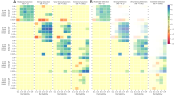
\includegraphics[width=1\textwidth]{figures/poly_panel_figure_2plots.pdf}
    \caption{Impact of Polygenicity on Populations' Survival. Panel \textbf{A} illustrates the effect of the number of contributing alleles (polygenicity) on populations' survival rates through the fitted logistic regression slopes between polygenicity and survivalship. Each colored square represents one slope/error value when all the reminaing parameters are kept constant as indicated in the figure, providing a comprehensive view of how polygenicity interplays with these factors. In panel \textbf{B} the survival rates of populations are superimposed with varying degrees of transparency, visually emphasizing areas of lower (less transparency) or higher mortality (more transparency). These plots highlight the critical importance of polygenicity, especially at the margins of survival, in shaping the evolutionary outcomes of populations.}
    \label{fig:poly_panel_figure}
\end{figure}

\begin{figure}[b]
    \centering
    \includegraphics[width=1\textwidth]{figures/meanfitness_varfitness_gen0to4.pdf}
    \caption{Mean Fitness and Fitness Variance at the Extinction Edge based on Genetic Architecture. Panel B depicts the mean fitness across two generations (Generation 0 and Generation 4) for varying levels of polygenicity, initial allele frequency range of contributing loci and heritability levels. Panel B illustrates the corresponding fitness variance for the same generations and genetic architectures.}
    \label{fig:meanfitness_varfitness_gen0to4}
\end{figure}

\begin{figure}[b]
    \centering
    \includegraphics[width=1\textwidth]{figures/mean_fitness_acrossgen.pdf}
    \caption{Evolution of Mean Fitness at the Extinction Edge based on Genetic Architecture. Changes in mean fitness across generation for different initial allele frequency and polygenicity of contributing loci and heritabilty levels.}
    \label{fig:mean_fitness_acrossgen}
\end{figure}

\begin{figure}[b]
    \centering
    \includegraphics[width=1\textwidth]{figures/var_fitness_across_gen.pdf}
    \caption{Evolution of Fitness Variance at the Extinction Edge based on Genetic Architecture. Changes in fitness varince across generation for different initial allele frequency and polygenicity of contributing loci and heritabilty levels.}
    \label{fig:var_fitness_across_gen}
\end{figure}

\begin{figure}[b]
    \centering
    \includegraphics[width=1\textwidth]{figures/metrics_boxplots-1.pdf}
    \caption{Caption of the figure.}
    \label{fig:metrics_boxplots}
\end{figure}

\begin{figure}[b]
    \centering
    \includegraphics[width=1\textwidth]{figures/metrics.pdf}
    \caption{Caption of the figure.}
    \label{fig:metrics}
\end{figure}


%% Supplementary figures 

\begin{figure}[b]
    \centering
    \includegraphics[width=1\textwidth]{figures/survivalshipforh2-1.pdf}
    \caption{Populations' survivalship across different values of polygenicity, initial allele frequency of contributing loci, strength of selection regimens and distance to new optimum.}
    \label{fig:survivalshipforh2}
\end{figure}

\begin{figure}[b]
    \centering
    \includegraphics[width=1\textwidth]{figures/survivalship_forpoly-1.pdf}
    \caption{Populations' survivalship across different values of heritability, initial allele frequency of contributing loci, strength of selection regimens and distance to new optimum.}
    \label{fig:survivalship_forpoly}
\end{figure}

\setcounter{figure}{0}
\renewcommand{\thefigure}{S\arabic{figure}}
\begin{figure}[b]
    \centering
    \includegraphics[width=1\textwidth]{figures/phenotypes_initial-3.pdf}
    \caption{Initial Phenotype Distributions Across Genetic Architectures. This figure presents the initial phenotypic distributions for populations with different levels of polygenicity, initial allelefrequency and heritability. Each plot shows the Kernel Density Estimate (KDE) of phenotypic values.}
    \label{fig:phenotypes_initial}
\end{figure}

\begin{figure}[b]
    \centering
    \includegraphics[width=1\textwidth]{figures/phenotypes_initial_onlymonogenic-2.pdf}
    \caption{ Initial Phenotype Distribution in Monogenic Architectures. This figure depicts the distribution of initial phenotypic values in populations where only one allele contributed to the trait value and varying initial allele frequency ranges and heritability values. The distribution is shown as a Kernel Density Estimate (KDE) of phenotypic values. This visualization highlights effect of heritability on low complecity architectures, where high heritability values normalize the phenotypes distributions.}
    \label{fig:phenotypes_initial_mono}
\end{figure}

\begin{figure}[b]
    \centering
    \includegraphics[width=1\textwidth]{figures/genetic_values_vs_lowheritability_difpoly.pdf}
    \caption{Comparative Analysis of Phenotype Distributions Across Various Polygenicity Levels Under Antagonistic Heritability Levels. Panel A illustrates the phenotypes' frecuency assuming a heritability of 1 for all combinations of polygenicity and initial allele frequency range for the trait contributing loci. Panel B presents the same range of polygenicity and initial allele frequency levels for the contributing loci but with a significantly reduced heritability of 0.1.}
    \label{fig:genetic_values_vs_lowheritability_difpoly}
\end{figure}


\section{Discussion}
\subsection{How to determine rapid evolutionary outcomes?}

Understanding the evolutionary dynamics of rapid adaptation is key, since it has direct application in many fields. From understanding invasive species invasion to harsh environments (Lee 2002; Lee and Gelembiuk 2008), applied evolutionary rescue for species at extinction risk, or even understanding medical concerning issues like the emergence of novel infectious diseases where genetic adaptation to a novel host is required (Holt and Hochberg 2002; Antia et al. 2003).

Rapid adaptation has been widely documented as shown in the examples listed in the introduction. But, this does not mean that it can always occur. The mentioned examples highlight the \textbf{potential}, in principle, for rapid adaptation to overcome environmental changes. However, the number of species that have not adapt to harsh and rapid environmental changes surely surpass  the short list of cases that have. Decades ago, in a theoretical work \citep{Gomulkiewicz1995-sj} conclude that regardless of the genetic model, populations with the necessary genetic variation to adapt may still often fail to do so in novel environments. 

In order to predict the evolutionary outcome and take concrete measurements and follow up actions, we first need to understand the key parameters playing a role in populations and species probability of extinction after a sudden environmental change. For example, it is now, widely known that the  probability  of  population  survival  increases  nearly  linearly  with  both  population  size  and  the number of exchangeable loci (diversity) . These, are  parameters that can be measured and would allow practical management decisions. 

\subsection{Genetic architecture is a key parameter defining evolutionary outcomes}

Particularyl, in this study, we focus on few key parameters of an adaptive trait genetic architecture: number  and initial frequency of contributing loci and heritability, which have controversial literature. 

According to the 'selective sweep paradigm' most studies from a decade ago have focus on the dynamics of a trait determined by a single locus that is sufficient to rescue a population exposed to an environmental shift (Hermisson and Pennings 2005;  Hermisson and Pennings 2005; Barrett and Schluter 2008). Gomulkiewicz \& Holt  originally examined a quantitative-genetic model and a one-locus model  and obtained qualitatively similar results in terms of evolutionary outcomes \citep{Gomulkiewicz1995-sj}.  Later on, Orr and Unckless, already highlighted the fact that it would be difficult for a single locus to adapt to rapid environmental change compared with the case for multiple loci where any one of them can rescue the population \citep{Orr2014-yn}. Later on,  on a theoretical work, Gomulkiewicz showed that increasing the number of loci can decrease the speed of adaptation and prevent the resultant rescue from extinction because selection per locus is weakened \citep{Gomulkiewicz2010-wr}, the opposite to what we found.

The big difference between their and our approach is the definition used for fitness. They, use an additive model of malthusian fitness at time $t$ as
\[
m_t = \sum_{i=1}^{n} \left( p_{t,i}^2 m_{AA,i} + 2p_{t,i} q_{t,i} m_{Aa,i} + q_{t,i}^2 m_{aa,i} \right)
\]
where  
$n = \text{Number of loci}$, $p_{t,i} = \text{Frequency of allele A at locus } i \text{ at time } t$, 
$q_{t,i} = \text{Frequency of allele a at locus } i \text{ at time } t$, $m_{AA,i} = \text{Fitness of the AA genotype at locus } i$,
$m_{Aa,i} = \text{Fitness of the Aa genotype at locus } i$,
$m_{aa,i} = \text{Fitness of the aa genotype at locus } i $. They define $A$ as the advantageous allele at the new environment, and hence selection acts on the other two genotypes, so $m_{AA,i} = \frac{r_{\text{max}}}{n}$, $\text{ } m_{Aa,i} = \frac{r_{\text{max}}}{n - \frac{s_i}{2}} $, and $m_{aa,i} = \frac{r_{\text{max}}}{n - s_i} $
Where $r_{\text{max}}$ represent the maximum population growth and $s$ the selection coefficient. From this, they derived $m_t = r_{\text{max}} - \sum_{i=1}^{n} s_i q_{t,i}$
Finally, they solve for s: 
$s = \frac{r_{\text{max}} - m_0 + \frac{2V_0}{r_{\text{max}} - m_0}}{n}$ Assuming, m0 (intitial fitness mean is constant) and V0 (intial variance mean) is constant. Finally the obatined s on  $T = \frac{2 \ln(\frac{s}{ns - r_{\text{max}} q_0})}{r_{\text{max}}(1 - q_0)}
$. T is the number of generations that it would take for the population to go from negative intial growth (population destined to go extinct wihtout adaptaiton) and recover, to tehn grow. Based on this, they conlcude that the more loci involed in the adaptation process, the weaker the selection at each of them and the larger it would take for the population to adapt. 

In our approach, fitness is a function of phenotype, and the same phenotype can be achieved with multiple genetic architectures. Furthermore, what genetic archtecture indeed determines is the initial fitness mean and variance, while they assume it is constant across genetic architectures.  \ref{fig:mean_fitness_acrossgen, fig:var_fitness_across_gen,  fig:meanfitness_varfitness_gen0to4}. We observe even more variation for high heritability levels (they assume heritability to be 1 throughout their model).

Finally, our results are in concordance with more recent work by, Kardos \& Luikart where they develop more realistic scenarios through simulations. They demonstrated that population extinction is less likely in models with polygenic architectures compared with models with large-effect loci due to higher short-term evolutionary potential \citep{Kardos2021-jd}. 

\subsection{Why polygenicity increases the odds of survival at the extinction edge?}
Based on our observation, increased trait polygenicity has a positive effect on the survivalship probability at the extintion edges (\ref{fig:poly_panel_figure}), and independently of initial mean and variance fitness, more polygenic traits reach higher mean  and variance fitness after only 10 generations (\ref{fig:mean_fitness_acrossgen,  fig:var_fitness_across_gen, fig:meanfitness_varfitness_gen0to4}). We argue that this results are based on two main things: 
\begin{enumerate}
    \item Polygenic architecture can generate exponentially more phenotypes, distributed in a more continuous manner. In polygenic architectures, the effect of each loci starts to be tiny on the overall phentoype, and the combinatorics of all loci, creating a continuous distirbution of phenotypes \ref{fig:genetic_values_vs_lowheritability_difpoly}. The opposite is true for monogenic architectures. Based on combinatorics, low polygenic architectures, can produce a lower number of resultant phenotypes, and their disitrubtion is hihgly dependent on the initial allele frequency of the contributing loci (\ref{fig:genetic_values_vs_lowheritability_difpoly}). This thight link between low polygenic architectures and initial allele frequency of contributing loci, end up in more disruptive distribution of pehnotpyes. This phenotypes, might or might not end up being adaptive to the new optimum. 

    \item Redundancy: One central property of the genetic architecture of polygenic traits is the general many-to-one relationship, a single phenotype corresponds to a larger number of genotypes. These genotypes are thus redundant with respect to the phenotype they produce and individuals can use different sets of alleles to produce the optimal phenotype. This has been already hihgligted by \citep{Orr2008-jl}. 
\end{enumerate}

\subsection{High heritability does not improve survival in low complexity traits}

Our results showed that at low polygenic architectures, heritability does not increase the chances of survivalship. Opposite to that, depending on the intial allele frecuency of the contributing loci, heritability might correlate negatively with survivalship. (\ref{fig:h2_panel_figure}).

Heritability is known as evolution's memory.  Selection operates on heritable traits. For a trait to evolve through selection, it must be at least partly heritable. If a trait that provides an advantage is heritable, it is more likely to be passed on to the next generation.  In this sense, our results are contraintuitive. Nevertheless, based on the stochastic dsitirbutions of phenotypes in the low polygenic architectures explained in the previous section, low heritability actually acts as continuzation of discrete phenotypes, filling in the gaps. Under high heritaiblity (when the phenotype is mainyl determined by the genetic value) low complexity architectures are very suseptible to the intial frequencys of the contributing loci to their trait. a decrease in the hertibability value, mkae the distribution of phenotypes to get more similar to what we observed in the high polygenicity case. Given them overall, just by chance or based on noise a higher overall porbability of survivalship. 

\subsection{Polygenicity is not intrinsically better}

As stated by Lande eary on 1983 adaptation from polygenic or monogenic traits is equaly feasible  \citep{Lande1983-kz}, and we believe so, under the assumption that they can both achieve the optimum trait value. We believe that if the trait value is adaptive, independent of its genetic architecture, it will have enough fitness and will allow the population to overcome extinction. Nevertheless, higher polygenic architecture will cover the phenotypic space in a more continuous and consistent manner, enhancing their odds to adaptation to further optima. 

We would like to hihglight, the fact that this is true under two main assumptions: the new optimum is on a reachable range and adptation is solely based on standing variation. This is quite important, since in an escenario where the new optimum value is out of range and standing genetic varaition wouldnt be enough to reach it, the opposite might be true. If the optimum is far enough, so the current population pehnotype disitrbutiun all its individuals would have 0 fitness in the new environemnt, scaping extintion would onty rely on de novo mutations. In this case, the number of mutations needed for a trait to adapt to a new far optimum, would be lees in the case of the low complexity architecture, while in the case fo the hihgly polygenic architecture, many mutations would be needed, to coordinate a new trait value. Based on this, we highlight that our results woudl be more applicable in a context of envrionmental shift that dont exceed a magnitude where the population would be completely maladaptive. This cases might be mostly seen with cliamte slowly but sustaintable changing, but not in cases for invasive species where the population might be completely maladaptive to teh new optimum. 

We conclude that, if the genetic variance exist to adapt to the new optimum, polygenic architectures show more robust adaptive capacity reaching further new optimum. Low polygenic architectures, might or might not adapt and are higly depdent on initial allele frequency of contributing loci. Overall, low polygenic architecture do not produce ''worst', they just produce less and disruptive distribted phenotypes. 

\subsection{Novel GWA across environments are needed to identify causal adaptive loci to different climates}

Our results show that current available tools are not yet suited for the identification of adaptive loci in the context of an E\&R experiment across environemnts in an an organisms with high self fertilization rates. 
The lack of recombination will lead to the formation genetic blocks are during polygenic selection under self fertilisation \citep{Hartfield2022-nc}. Adaptive loci will increse in frequency, but will take with them a block of neutral hitchickers. This is particularly complicates the identification of adaptive loci. 

Nonetheless we believe that this problems can be overcome with the developing of new statistical approaches. 

\subsubsection{Final comments}
Our model is subjective, and it lives under simplifying  assumptions, while also igorning other biologically relevant parameters. But we also believe that the simplicy allows to hihglight key interactions. We did not model different demographic scenarios, nor population sixes, we didn't explore further in a two trait models to include higher level interactions like epistasis, or pleiotropy. 

We also know that teh cost of using real genetic data from A. thaliana, makes oru results subscriptive to a population with low outcrossing rates, and hence low recombinations rates. Also, because A. thalina  reproductive excess may be able to accommodate high levels of mortality without a decrease in adult population size if growth rate is not reduced to below replacement (Crow 1970, paper from moi).


On this set of simulations we have inspired ourselves on the experimental set up of GrENE-NET and on the biology of A. thaliana. 
Polygenic selection has been extensively studied in models assuming random–mating. Yet many species self fertilise to some degree, which incurs changes to genetic diversity, recombi- nation and genome segregation. Studying selfing might be of paritucalr importance in agricultural relvant crops. Even though, low complexity or hihgly polygenic architecutres haven described in mixed mating organissm like Mimulus  guttatus;  Troth et  al. (2018) but also in hihgly selfing selfing plant Arabidopsis  thaliana (Zan  and  Carlborg  2018;  Exposito-Alonso et  al. 2018;  Tsuchimatsu et al. 2020; Wieters et al. 2021), but studies of genetic architecture implication of the evolutionary outcome have only been described in models assuming random–mating, and we could ppnly find one work where the evolutionary outcomes of selfing was explored \citep{Hartfield2022-nc}.




\subsection{to do}
- create figure for var in fitness to cite
- make sure all figures abor fitenss variance and fitness mean are about the same little square 

\subsection{extra}
explore if in the polygenic or monogenic adaptation the alleles of high or low effect persisted

I should calcualte the 'selection limits' bascialyl the difference between mean phenotypes at gen 4 - mean pheno gen 0 
Calculation of L0: L0 is calculated as the difference between the predicted mean phenotype at ten generations and the mean phenotype at the beginning of the simulation.
Regression Analysis: A regression analysis is used to measure the relationship between L0 and population viability. Specifically, generalized linear models (GLMs) with a logit link function in R are used, with population persistence as the response variable, coded as 0 for extinct populations and 1 for populations that persisted

compare the r squared of the casual with the one from the non causal

\bibliography{paperpile} % Bibliography

\end{document}
